%----------------------------------------------------------------------------
\chapter{Optical character recognition}

This chapter focuses on the OCR (Optical character recognition) part of the ALPR process. I propose a lightweight algorithm that is part of a vehicle identification pipeline capable of running on Android smartphones.

Optical character recognition consists of character localization- and classification. It is responsible for producing machine-encoded text from a text image. First, character segmentation is applied, separating individual characters on the image. The name is a bit misleading as it can be object detection or semantic segmentation. Then follows classification, which is about outputting one machine-encoded character based on an image of a single character.

There are two main approaches regarding Optical Character Recognition with deep learning. Object detection can be used to locate individual characters on images. This solution outputs a character score for each detected box, instantly recognizing tokens in multiline plates. However, there are significant drawbacks in the context of OCR\cite{CTCexp}:

\begin{itemize}
  \item Annotating real-life datasets on a character level is time-consuming.
  \item Detectors usually struggle with small objects (like characters in text).
  \item The outputs are character scores, and therefore further pre-processing is needed to get the final text from it.
  \item When using fixed boxes, a single character can trigger multiple positions. It is possible that ``GGOO'' is the prediction because the ``O'' is wide. In that case, we must remove all duplicate tokens. Nevertheless, it can be that the original text would have been ``GGO''. Then removing the duplicates produces a wrong result.
\end{itemize}

Another approach can be the sequential feature extraction with convolutional and recurrent layers guided by Connectionist Temporal Classification\cite{CTC}. In this solution, the convolutional part extracts the necessary features. Then the recurrent part processes them sequentially to output a probability for each time step. The main advantage over the object detection approach is that only an image and the target text need to be provided; CTC handles the rest. Therefore, character positions and width are ignored, which makes it easier to label real-life datasets. An output sequence of a CRNN can be easily translated into a text with either the Greedy or Beam search algorithms, as CTC also indicates the end of the characters with a specific token. However, these solutions can process images along one axis (practically horizontally); therefore, they cannot recognize multiline blocks in standalone versions.

Different approaches exist to convert CRNNs into multiline recognizers. The classical solution can be the Scale Space Technique for Word Segmentation\cite{ScaleWordSeg}, which outputs block positions. It performs relatively well (87\%) on handwritten papers. For multiple text block recognition, both an object detector or an image segmentation model can be used first, and their outputs then fed into the CRNN. However, this solution is wasteful as an image must be processed multiple times, and low-level feature extractions are not shared across individual networks. Recently, Wojna et al.\cite{Attention-basedExtract} proposed an end-to-end model with an attention mechanism. OrigamiNet\cite{OrigamiNet} introduced a one-step model by learning to unfold, transforming existing CRNNs into multiline recognizers. Other approaches still exist, like proposed by WPOD-NET\cite{WPOD-NET}, where a modified YOLO detector is used for OCR purposes.

\section{Data}

An adequate amount of data is required to train a deep learning algorithm. There were only a few number plate datasets for object detection (which were missing text labels). The OCR sets neither satisfied the search as they were too specific in domains like handwriting recognition or housing numbers. A good option where there are 15 million annotated images is the database of platesmania.com\cite{PlatesMania}. However, their API access proved to be expensive even for chunks of 50,000 images, as is their offline license plate generator script.

The nature of license plates varies between countries or even provinces. There are plenty of structures, colors, and fonts (like the modified Mittelschrift in Hungary or the Mandator font in the UK). There can be single-line vs. multi-line versions. Some countries use non-Latin alphabets (like China or Egypt), which makes the task even harder. Figure \ref{fig:plates} shows some example license plates. Taking these into account, I aim to recognize Latin alphabet characters; 17 currently used number plate fonts have been collected from Australia, North America, and Europe.

\begin{figure}[htb]
 \centerline{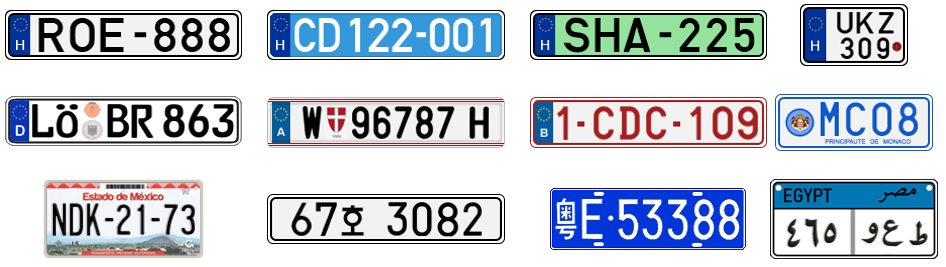
\includegraphics[width=1.0\columnwidth]{.//Figure/OCR/plates.png}}
 \caption{License plates from Hungary (1st row), Europe (2nd row), and other continents (3rd row).}
 \label{fig:plates}
\end{figure}

A few characters are traditionally hard to distinguish in the Latin alphabet, like 0-O-Q, 1-I, or 8-B. This issue is often eliminated by prohibiting letters and numbers on the same character position. However, as plate structures can vary even in a single country, this is not a general solution. Moreover, two different characters may be the same in a font (like 0-O in the Mandatory) or across different fonts. Therefore, I decided that the unique items to distinguish are 0-9 and A-Z excluding O, plus the hyphen (10 + 25 + 1 characters). Other difficulties arise from picture quality and visibility aspects (lighting, contrast, rotation, motion-blur). This diversity suggests a general OCR model has the edge over systems based on hand-crafted feature extraction for each plate type.

For this reason, I implemented a data generator, which approaches the task at the character level. It uses three types of resources to create an output: a list of characters to generate random text, fonts, and overlay images to mimic dirt, ice, and other phenomena. The generator also handles character-level bounding boxes to be converted to output detector training data, producing multiple text blocks. Creating one $200\times200$ RGB image takes roughly 30 ms without bounding boxes and 61 ms with them. The generator applies data augmentation techniques to enrich data diversity. Algorithm \ref{alg:data_generator_pipeline} shows the individual steps of the pipeline.

\begin{algorithm}
\caption{Data generator pipeline}
\label{alg:data_generator_pipeline}
\begin{algorithmic}[1]
 \STATE \textbf{procedure} Generate($args$)
 \STATE random font and image overlay from $args$
 \STATE $bckgColor$ = random value [0...255] in every channel
 \STATE $image$: create with defined dimensions from $args$ and $bckgColor$
 \STATE $generatedTexts$ = $args[numBlocks]$ random texts in the range of 1...10.
 \STATE $lastBoxCoords$ = [0,0,0,0]
 \STATE $insertedTextIndices$ = []
 \FOR{$text$ in $generatedTexts$}
 \STATE $textColor$ = text and background colors must have at least 20\% diff in one channel (randomly selected which channel satisfy this)
 \STATE $textImage$: create text image from $text$, with a background color identical to $bckgColor$
 \IF{$textImage$ is bigger than $image$ in any dimension}
 \STATE $textImage$: resize to fit onto the $image$
 \ENDIF
 \STATE $textImage$: resize ratio with a value in the resize range (typically 0.85...1)
 \STATE $textImage$: random aspect ratio change, heigh, and width offset
 \IF{($lastBoxCoords[3]$ < $boxYstart$) || (($lastBoxCoords[2]$ < $boxXstart$) \&\& ($lastBoxCoords[1]$ < $boxYstart$))}
 \STATE $image$ += $textImage$
 \STATE $lastBoxCoords$ = [$boxXstart$, $boxYstart$, $boxXend$, $boxYend$]
 \STATE $insertedTextIndices$ += currentBoxIndex
 \ENDIF
 \ENDFOR
 \STATE $image$: random rotation and perspective transformation
 \STATE $image$: resize to the required size
 \STATE $image$ += random overlay with offset and rotation
 \STATE $image$: random brightness, contrast, sharpness, gaussian blur (within $args$ constraints)
 \STATE $image$: downscale between a range from $args$, then scale back
 \STATE $image$: normalize from [0...255] to [-1...1), convert to float32
 \STATE $label$ += $text$ which Id is in $insertedTextIndices$
 \STATE $label$: encode $label$ to a number label with dictionary from $args$
 \STATE return $image$, $label$
\end{algorithmic}
\end{algorithm}

As the validation samples are also generated, the images must be equally distributed across different evaluation sets. A single evaluation epoch is set to contain 10,000 images. With this size, there is a maximum of +/-0.015 deviation in loss across multiple validations. Figure \ref{fig:generated} shows some random one-line generated sample.

\begin{figure}[htb]
 \centerline{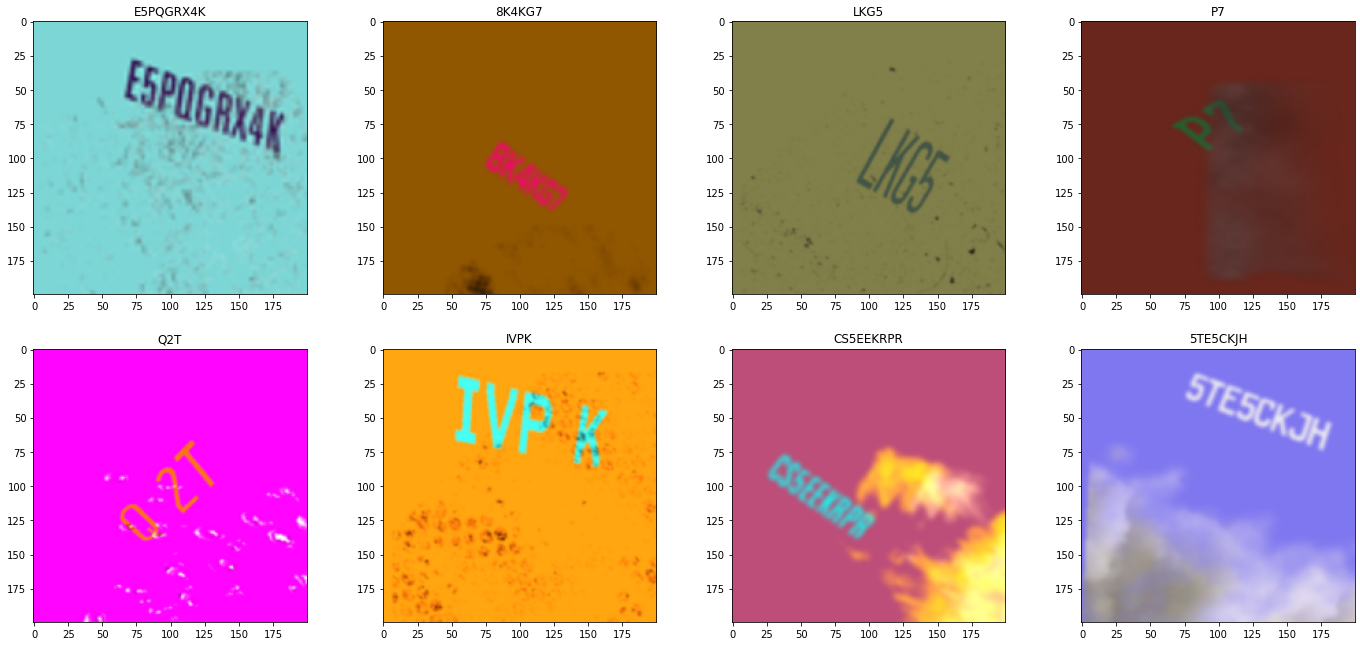
\includegraphics[width=1.0\columnwidth]{.//Figure/OCR/generated.png}}
 \caption{One line generated samples with labels on top. Hard overlays have been removed from the validation set so that the completely illegible characters do not affect results.}
 \label{fig:generated}
\end{figure}

\section{Sequential approach}

My first OCR approach is based on feed-forward recurrent convolutional networks (CRNN) that produce fixed-size arrays of character probabilities.

\subsection{Connectionist Temporal Classification}

Connectionist Temporal Classification\cite{CTC} is used to compute model loss. The cost function has a barely documented Keras implementation, which I wrapped into a layer to make it easily detachable after training. This layer has two inputs: model prediction (\textit{batch\_size, max\_timesteps, num\_characters}) and ground truth encoded as numbers (\textit{batch\_size, max\_len}). Besides the 36 identifiable items, two more numbers are indicating the non-character token and the unknown character. Inputs must be the same length in a single batch. If a label's text is shorter than the maximum length, padding is expected with non-character tokens. The padding ensures that the model can be trained with greater batches than one, as multiple labels can be merged into a single, same dimensional array. The layer deduces the length of each label at runtime before computing its cost. To do that with arbitrary batches, I had to put a loop into the layer. The implemented TensorFlow loop is 30\% slower than the Python counterpart, but it can be placed on a TensorFlow graph.

\subsection{Building blocks}

A custom convolution layer is defined with Convolution $\rightarrow$ Nonlinearity $\rightarrow$ Dropout $\rightarrow$ Batch Normalization (Figure \ref{fig:blocks}). These types of layers are stacked on top of each other in the residual blocks. The implementation allows to specify the type of activation function, the proportion of dropout, and whether to use Batch Normalization or not (when enabled, it adds bias to the output, so the convolution operation's bias is disabled in that case). Every convolution operation uses ``SAME'' padding. It applies padding so that the whole input gets fully covered by the filter and specified stride. The name comes from that, for stride 1, the size of the output is the same as the input. This partly solves the skewed kernels and feature-map artifacts issue induced by the operation\cite{PadBlindSpot}.

The main parts of the network are the residual blocks which consist of three components. The residual stage contains an arbitrary number of convolution layers with the same input/output size and channels. This block of layers is defined with a skip connection between the input and the output to overcome the vanishing gradient problem, which that means the block's input directly influences its output through a ``gradient highway'', not just through convolutions. After that, an upscaling convolution layer doubles the number of channels (it is the only layer that gradients cannot bypass; therefore, it is a bottleneck). It is followed by spatial downscaling by a factor of two with pooling. The structure is illustrated by Figure \ref{fig:blocks}. In this configuration, a block with input dimensions (height, width, channels) has an output of \((\frac{height}{2}, \frac{width}{2}, channels\times2)\). My implementation was inspired by the ResNet\cite{ResNet} architecture.

\begin{figure}[htb]
 \centerline{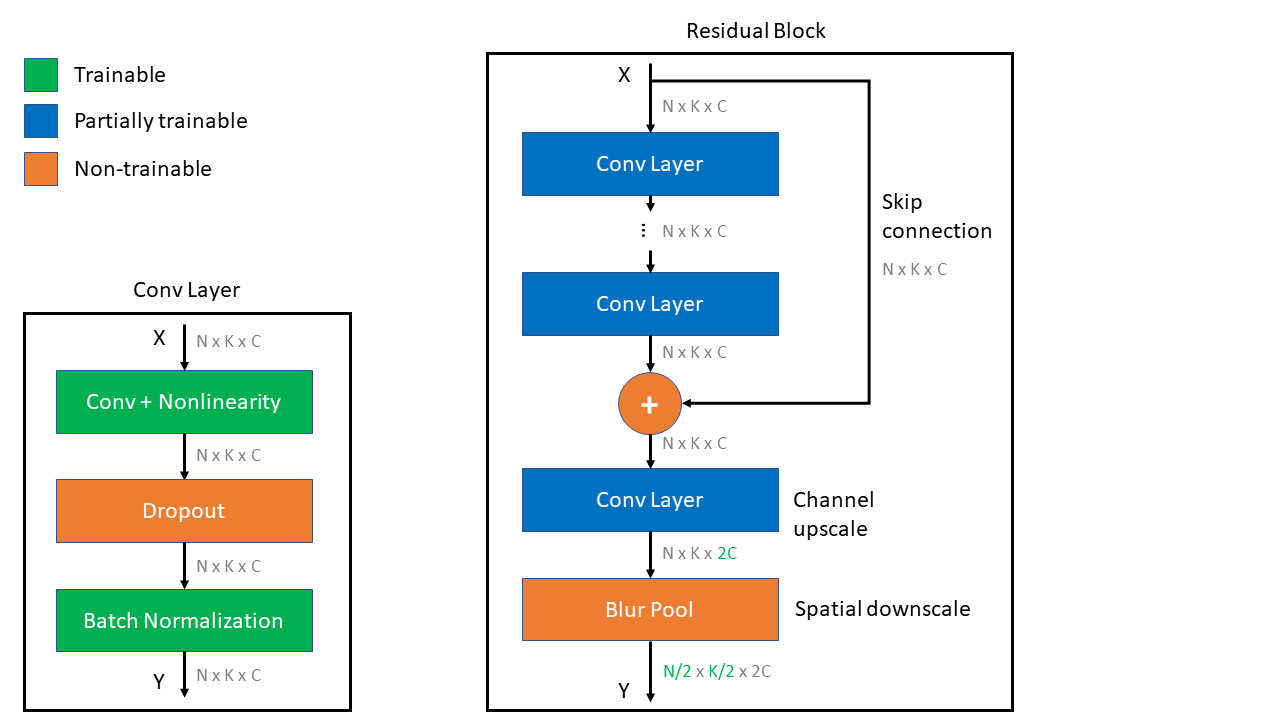
\includegraphics[width=1.0\columnwidth]{.//Figure/OCR/blocks.png}}
 \caption{Network building blocks with the convolution layer (left) and the residual block (right).}
 \label{fig:blocks}
\end{figure}

In the recurrent part of the network, two Long Short-Term Memory\cite{LSTM} layers are stacked on top of each other responsible for sequential processing. At the time of this work, GRU TensorFlow Lite support was unavailable, so I could only use LSTM for smartphone inference. In the network's first layer, the height and width dimensions of the input are swapped so that the width is the first dimension in the model. Thus, recurrent layers process inputs horizontally. A dense layer follows the last LSTM layer with a dimension of (${input\_width}\times{downscale\_factor}$, \textit{num\_characters}), which is the network's output matrix. The high-level operation of the model is illustrated in Figure \ref{fig:processing_steps}.

\begin{figure}[htb]
 \centerline{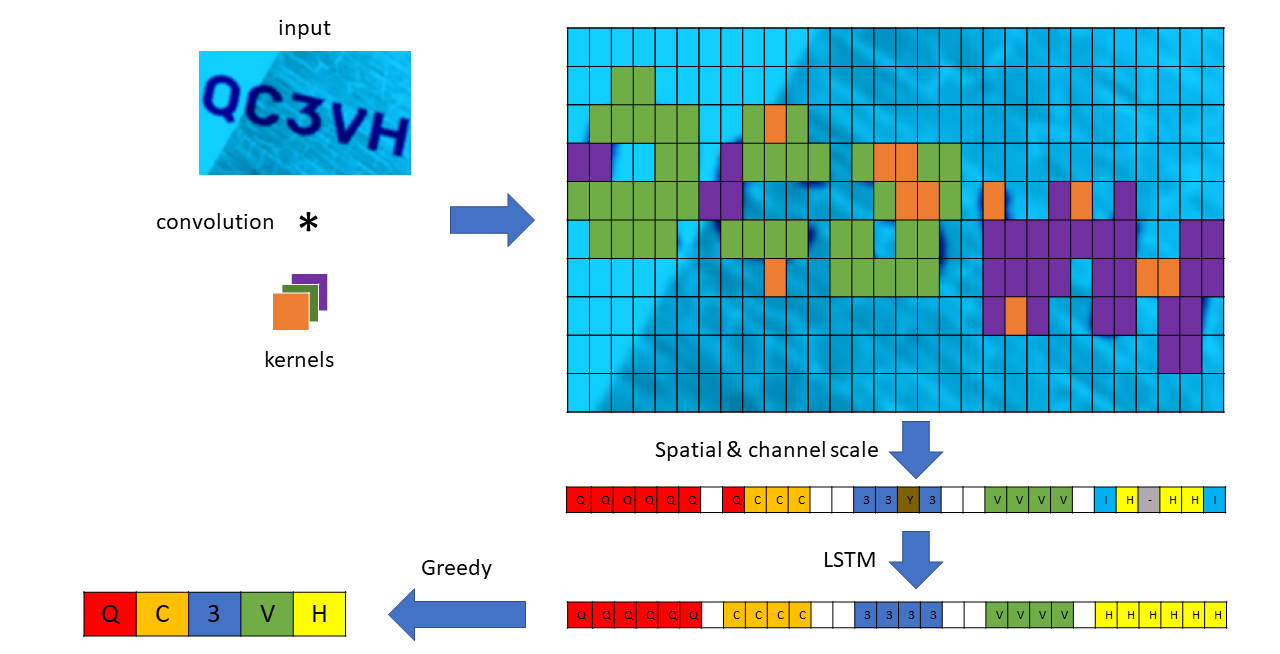
\includegraphics[width=1.0\columnwidth]{.//Figure/OCR/processing_steps.png}}
 \caption{Simplified representation of the network's key processing steps.}
 \label{fig:processing_steps}
\end{figure}

The best model has a downscale factor of three (number of residual blocks) and an input image width of 500 pixels, which means 63 steps overall. One window has a width of 8 pixels. Each window must be assigned to a real or an empty character token. It means that net 31 characters can be recognized to have enough space for characters and empty tokens in the output matrix.

\subsection{Greedy search}

In training, the CTC layer handles raw model outputs and ground truth labels, then calculates loss to backpropagate. However, this is not required for inference. Multiple approaches are available to decode raw outputs of the last dense layer. The Greedy solution keeps the maximum index at each step, then merges the same tokens between empty tokens. This way, multiple recognitions triggered by the same character are eliminated. The next step is to remove the empty tokens and decode the sequence with the model's vocabulary. That step produces the final text. Other approaches, like Beam search, iteratively create text candidates, arranges them based on their probability scores, and keeps the best ones after every iteration. The most probable beam at the end is returned as a result. This algorithm can be highly computation-intensive depending on the number of beams. Word Beam Search\cite{WordBeamSearch} takes this idea to another level: it constrains beams with a prefix tree of existing words. This solution can be helpful in situations where the words to recognize are from a specific vocabulary, but in the case of plate recognition, such a semantic assumption does not help. For these reasons, I implemented the Greedy algorithm.

\subsection{Experiments}

As a starting point, the model is trained with two residual blocks with a single convolution layer in each. The first block starts with 32 input channels, and the batch size is 8. Adam optimizer\cite{Adam} is used with the default parameters (\({1} \times {10^{-3}}\) learning rate). One epoch is equal to 100,000 images, and early stopping is applied with five epoch patience. This model reached the optimum after 13 epochs with a validation loss of 0.2298. I tried different batch sizes to find the most optimal as shown in Table \ref{tab:batch_sizes}.

\begin{table}[htb]
\caption{The effect of batch sizes. Smaller batches converged faster at the beginning of training, but their improvement flattened out earlier at worse sub-optimal points. Batch size 128 was the largest that could fit into the memory.}
\label{tab:batch_sizes}
\noindent
\centering
\begin{tabular*}
{\columnwidth}{@{\extracolsep{\stretch{1}}}*{3}{r}@{}}
    batch & epochs & loss\\ \hline
    8 & $8$ & $0.2121$ \\
    16 & $29$ & $0.1545$ \\
    32 & $22$ & $0.1134$ \\
    64 & $55$ & $0.0855$ \\
    128 & $51$ & $\textbf{0.0848}$ \\                   
\end{tabular*}
\end{table}

\subsubsection{Shift-invariance}

Zhang et al.\cite{Shift-Invariant} pointed out that modern CNNs lack shift-invariance since max-pooling, average-pooling, and strided-convolution ignore Nyquist's sampling theorem. The proposed solution is the use of blur-pooling, where spatial downsampling happens (Figure \ref{fig:anti_aliasing}). I implemented blur-pooling with separable kernels and replaced all the other pooling layers with them. Although they claim that the solution is compatible with the layers listed above, I wanted to keep the number of layers as low as possible. The shift-invariant model slightly improved in loss, but a lot in the speed of convergence. Therefore, I continued to work with this model as the new benchmark.

\begin{figure}[htb]
 \centerline{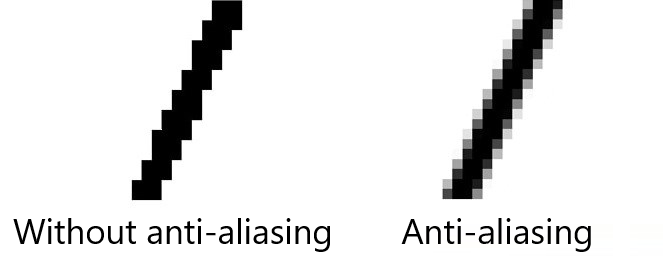
\includegraphics[width=0.6\columnwidth]{.//Figure/OCR/anti_aliasing.png}}
 \caption{The effect of anti-aliasing when scaling down a sloped line. Blur-pooling prevents the appearance of too sharp artifacts.}
 \label{fig:anti_aliasing}
\end{figure}

\subsubsection{1D convolution}

I experimented with using 1D convolutional layers instead of the LSTM cells. This way, the model does not have any recurrent part, only residual blocks with convolutions. The more straightforward structure without loops results in faster runtimes. However, the training became significantly longer, and the final result lagged behind the benchmark (0.08 vs. 0.1). The primary source of error was that one character triggered multiple different classifications based on the sequential processing's actual position. While LSTM can effectively smooth out 1D feature maps (``OCOO'' $\rightarrow$ ``OOOO''), it looked like 1D convolution had a more challenging time. Therefore, I no longer used this approach.

\subsubsection{Hyperband optimization}

Hyperparameter optimization has been realized with the Hyperband algorithm\cite{Hyperband}. Another option considered was Bayesian optimization. I chose the former because adaptive Bayesian methods do not handle discrete, independent, unordered values well, and training would have lasted longer (since one configuration is done when the model training stops). Hyperband is a fast guided random search that works like a knockout sports competition: it generates combinations and trains them for a few epochs. After that, the top-performing part of the models is trained further, while the others are discarded. The iteration repeats until all the remaining models stop learning or there is a clear winner. 

Hyperband strongly filters models based on early training performances. Therefore, variable batch size or learning rate was not possible with this algorithm because smaller batches tend to outperform larger ones initially, but not in the long run. The selected parameters to optimize were the number of features of the first block (which is then doubled by every consequent block), kernel size, whether residual connections and batch norm layers are needed, dropout rate, number of blocks, convolutional layers in blocks, and type of activation function. A batch size of 32 was applied during training with every model, as instances with more blocks and layers should also fit into memory. Therefore, the previous batch 32 model served as a baseline. The best configurations found by the optimization algorithm are shown in Table \ref{tab:top3}. Sample inference results can be seen in Figure \ref{fig:inference_sequential}.

\begin{table}[htb]
\caption{Top 3 configurations found by Hyperband. Only the top 2 and the baseline were trained until convergence (3rd model training has been stopped earlier). Columns: model, features, kernel, residual, batch norm, dropout, blocks, layer per block, activation, epochs, loss.}
\label{tab:top3}
\noindent
\centering
\begin{tabular*}
{\columnwidth}{@{\extracolsep{\stretch{1}}}*{11}{r}@{}}
    model & feat & ker & res & bn & drop & b & l & act & epochs & loss\\ \hline
    1st & $64$ & $3$ & $\checkmark$ & $\checkmark$ & $0.09$ & $3$ & $3$ & ReLU & $39$ & $\textbf{0.0753}$ \\
    2nd & $64$ & $5$ & $X$ & $\checkmark$ & $0.2$ & $2$ & $2$ & ReLU & $35$ & $0.0862$ \\
    3rd & $64$ & $3$ & $X$ & $\checkmark$ & $0.3$ & $2$ & $3$ & ELU & $15$ & $0.1554$ \\
    baseline & $32$ & $3$ & $\checkmark$ & $\checkmark$ & $0.1$ & $2$ & $1$ & ReLU & $22$ & $0.1134$ \\           
\end{tabular*}
\end{table}

\begin{figure}[htb]
 \centerline{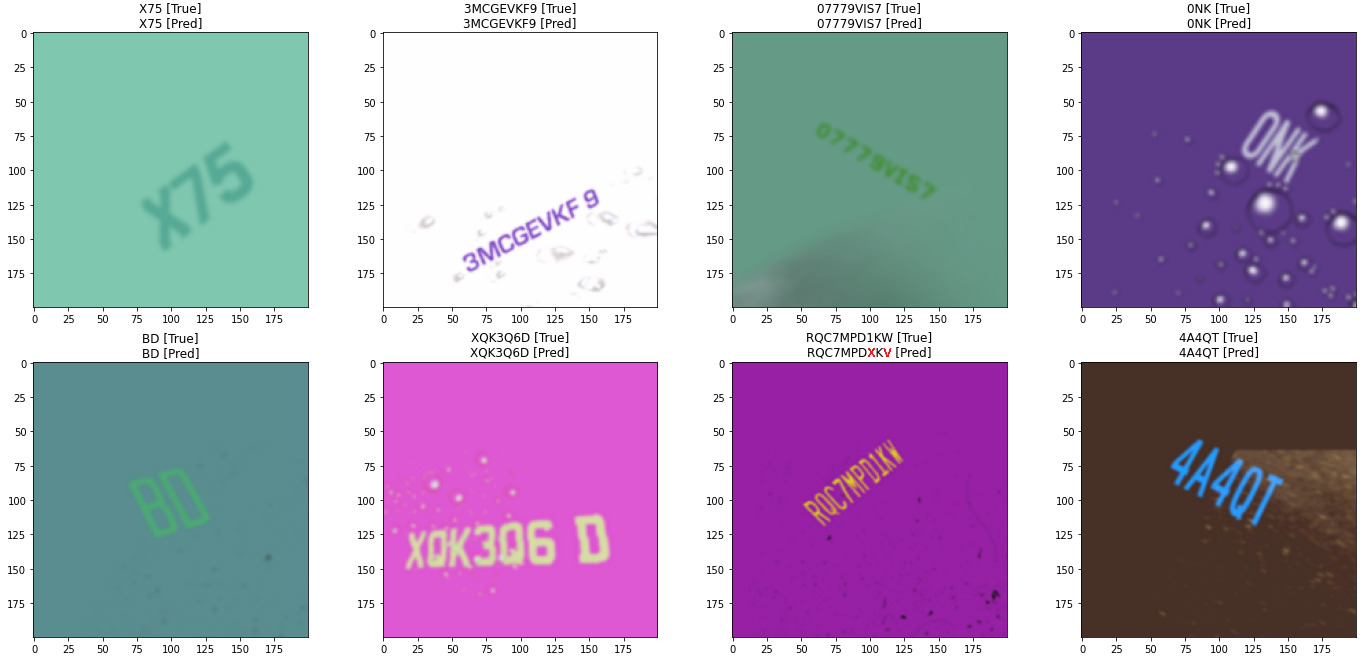
\includegraphics[width=1.0\columnwidth]{.//Figure/OCR/inference_sequential.png}}
 \caption{Inference results of the best performing network. Incorrect characters are marked as red.}
 \label{fig:inference_sequential}
\end{figure}

\subsection{Multiline recognition}

There are numerous approaches to process number plates with multiple lines. One can be the usage of object detection to detect individual text blocks on an image. One powerful model based on this approach is the CRAFT\cite{CRAFT} text detector. Another approach is text segmentation, which is not necessarily done by neural networks. In both cases, however, the recognition of text blocks and characters are separated steps and the weights used for them are not shared. I experimented with a model that merges these steps. The key idea is to add some layers to the end of the network that learns to unfold the two-dimensional feature map into a tall, one-dimensional feature sequence. This approach changes the main axis (the horizontal reading of text changes to process vertical features). To accomplish this, I implemented a modified Origami\cite{OrigamiNet} module that includes convolution layers and resizing with bilinear interpolation. The pseudo code of the module is shown by Algorithm \ref{alg:unfolding}.

 \begin{algorithm}
 \caption{Pseudo code of the Unfolding module.}
 \label{alg:unfolding}
 \begin{algorithmic}[1]
    \STATE \textbf{procedure} Unfolding($inDim, inChannel, outChannel, numBlocks, numLayers$)
    \STATE vertical = inputDim[0]
    \STATE horizontal = inputDim[1]
    \FOR{$i = 0$; $i$ $<=$ $numBlocks$; $i$++}
    \STATE vertical *= 2
    \STATE horizontal /= 2
    \STATE Resizing(vertical, horizontal, interpolation=bilinear)
    \FOR{$j = 0$; $j$ $<=$ $numLayers$; $j$++}
    \STATE Conv(inChannel, inChannel)
    \ENDFOR
    \ENDFOR
    \STATE Conv(inChannel, outChannel, (1, 1), (1, 1))
    \STATE xDownFactor = pow(2, $numBlocks$)
    \STATE xRemain = inDim[1] \% xDownFactor > 0
    \STATE xLastKernelSize = (inDim[0] // xDownFactor) + xRemain
    \STATE Conv(outChannel, outChannel, (1, xLastKernelSize), (1, xLastKernelSize))
\end{algorithmic}
\end{algorithm}

The original solution was not ideal for this task. I had to remove the recurrent part of the original network (LSTM layers) because they introduced instability while training. I replaced pooling with strided convolution, increased the number of resizing steps, reduced the spatial rescaling ratio, and increased the number of convolution layers. After these modifications, the module started working as intended. The best loss was 0.9517 on images with a maximum of five rows of texts after 73 epochs (0.0991 on single line images). It is far from an optimal solution, but all I had to do is to add a module to the end of an existing model. Unfolding also scales well, as the runtime does not change even when processing multi-row text images.

However, unfolding has its drawbacks. The original model had a size of 640 KB, while this module increased it to 3.138 MB. Multiplying the size of a model already reading single-line texts five times seems wasteful (even so, it is less than using a separate detector and a single line recognizer). Another problem is that unfolding struggles with rotated texts. It jumps through the lines while reading when rotation is close to 45 degrees. Therefore, in my opinion, this solution is not adequate for this task unless I apply an extra horizontal transformation step.

\section{Object detection approach}

RCNNs are fast and efficient on single-line texts but not ideal for multiline ones. To solve this, text block segmentation or detection can be used, which means an extra operation in the pipeline. Histogram-based text block segmentation can work, as the blocks are well separated in the case of license plates, but this is less effective on rotated number plate images. To remedy this, a license plate rectification operation is needed. To keep the number of processing steps low, I tried to solve the OCR task by character-level object detection, which can immediately handle multi-line texts.

I implemented the object detector from scratch for this task instead of using the TensorFlow Object Detection API. The API constraints a few things, like data encoding, available architectures, and usable backbone networks. With my implementation, I could understand the underlying concepts more thoroughly, and I could fine-tune the whole process at a lower level. 

I implemented a RetinaNet-based solution. I choose this architecture because the FPN provides multi-scale feature map outputs and the loss function that handles the class imbalance problem. It is also beneficial because of the decoupled classifier- and regressor heads, which add minimal latency but improve accuracy. I started with predictor heads each containing two convolutional layers, similar to the original publication. RetinaNet is an anchor-based detector, so I gained insight into this kind of operation during the implementation. The object detector training minimizes the loss function, but the evaluation protocols help understand how the algorithm performs at localization, classification, and general detection for different object sizes. Object Detection API's evaluation protocol implementation is deeply embedded in the API. It cannot be used as a standalone module. The whole API would have been added as a dependency to use their protocols, which I wanted to avoid. Due to time constraints, I could not implement a proper evaluation protocol, I used localization- and classification losses to draw conclusions.

\subsection{Experiments}

As a baseline, I created a small custom CNN as a backbone. I considered the original ResNet50 too complex for this task because we only need to detect characters that are not as complex and diverse objects as vehicles. The CNN has the following structure: at the beginning, a few feature blocks deepen the feature map but keep the input size. The subsequent spatial blocks keep upscaling the input feature maps by two while downscaling them spatially by the same factor. Each spatial block has an arbitrary number of convolutional layers inside with a residual connection between them. The last convolutional layer does the channel upscaling, meaning that the skip connection cannot bypass that layer, similarly to Figure \ref{fig:blocks}. I used the last three different-sized convolutional feature maps from the backbone as the inputs of the FPN. I used the input of $256\times256$ because, with the power of two input sizes, both pooling and nearest-neighbor downscaling (within the FPN) have the appropriate output size (the residue is treated differently, which is a problem in the case of inputs not in the power of two). An overview of the model is illustrated in Figure \ref{fig:starter_detector}.

\begin{figure}[htb]
 \centerline{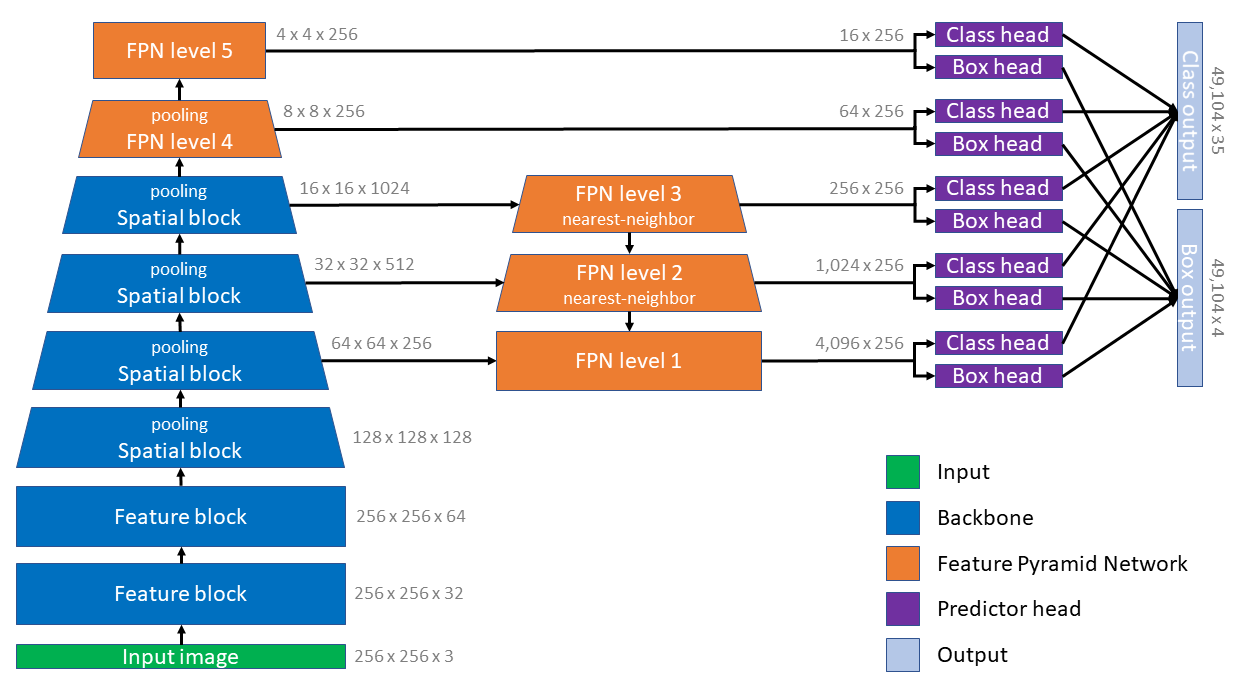
\includegraphics[width=1.0\columnwidth]{.//Figure/OCR/starter_detector.png}}
 \caption{The starter detector model. The predictor heads multiply the number of predictions by nine because of three different aspect ratios and three different scale ratios per anchor position.}
 \label{fig:starter_detector}
\end{figure}

\subsubsection{Loss and anchor configuration}

The default RetinaNet implementation uses anchor boxes of sizes \textit{32, 64, 128, 256, 512}. As the input images are only $256\times256$ pixels, I had to modify this. I used anchor boxes of sizes \textit{16, 32, 64, 128}, and \textit{256}. Similarly to the original configuration, I used three different aspect ratios \((\frac{1}{2}, \textit{1, 2})\) and three scale ratios \((\textit{0}, \frac{1}{3}, \frac{2}{3})\) for each anchor box size. With this configuration, the model had 49,104 anchor boxes for $256\times256$ inputs. The smallest anchor box the model can find is 16 pixels wide or long. This is \(\frac{1}{16}\)th of the input size. I consider it small enough because the input image is a license plate snippet, roughly 10-14 times as wide as one character on it. Thanks to the scale ratio, slightly smaller boxes can still be detected.

The models did not output any box prediction at the first few training sessions. It turned out that the loss function needed other parameters. The first problem was that the localization loss dominated the total value: there are 36 different classes in the OCR task, but the original COCO dataset has 80. An erroneous classification is more severely penalized if there are more classes by focal loss. I multiplied the localization penalty by 0.6 for downscaling. The other problem was that values for well-classified samples and wrongly empty-classified ones were very similar. The models learned to output nothing, thus minimizing the error. I tried different values to widen this gap and chose 0.85 and 1.2 for alpha and gamma parameters (instead of the original 0.25 and 2.0). After these modifications, the models could learn predicting boxes.

\subsubsection{Backbone}

I wanted to use as small network as possible. I tried a backbone with four convolutional layers as a starting point. This model could only localize huge boxes properly. This was because two convolutional layers could not generate a feature map that could be used to localize and classify objects. As I increased the number of layers, the detector got better. I added two feature blocks with one convolutional layer at the beginning of the network. After four layers, the starter model could output proper predictions (the last feature map responsible for huge objects). Increasing the number of layers helped the model converge, but the number of parameters got huge: I constrained the maximum output feature map in 512 dimensions to keep it low. In my opinion, this amount was enough to distinguish 36 classes properly.

I tried different feature map dimensions in the first convolutional layer; this value is then doubled for each block. The dimensions were \textit{16, 32}, and \textit{64}. The best results were with the value 32, but a model with only a 16-dimensional feature map produced similar results. Since this value significantly affects the size of the network, I chose the lowest because the deeper feature maps did not substantially affect performance as shown in Table \ref{tab:1st_feature_dimensions}.

\begin{table}[htb]
\caption{Detectors with different 1st layer feature dimensions.}
\label{tab:1st_feature_dimensions}
\noindent
\centering
\begin{tabular*}
{\columnwidth}{@{\extracolsep{\stretch{1}}}*{3}{r}@{}}
    1st feature map dimension & epochs & loss\\ \hline
    16 & $22$ & $1.4052$ \\
    32 & $26$ & $\textbf{1.4026}$ \\
    64 & $28$ & $1.4112$ \\         
\end{tabular*}
\end{table}

Next, I tried different feature map dimension constraints because this greatly influences the number of parameters. I experimented with values \textit{512, 256}, and \textit{128}. Training a model with 256 maximum feature dimensions did not decrease performance, but the model with only 128 could not achieve the same error rate. Hence, I chose 256 as the upper limit.

\subsubsection{Shift-invariance}

Initially, I used all the models with max-pooling. I experimented with the custom implemented blur-pooling layers, which worsened the performance in this case. I don't know the exact reason of this, but it could probably be that the feature edges of different objects got too blurred. This was not a problem with sequential models, where a character usually triggered multiple parts in a sequence, which CTC loss could handle. In object detection, it caused trouble in object localization. Therefore, I used max-pooling in the following models. Figure \ref{fig:blur_vs_max_pool} shows the effect of different pooling layers applied to an image containing larger objects.

\begin{figure}[htb]
 \centerline{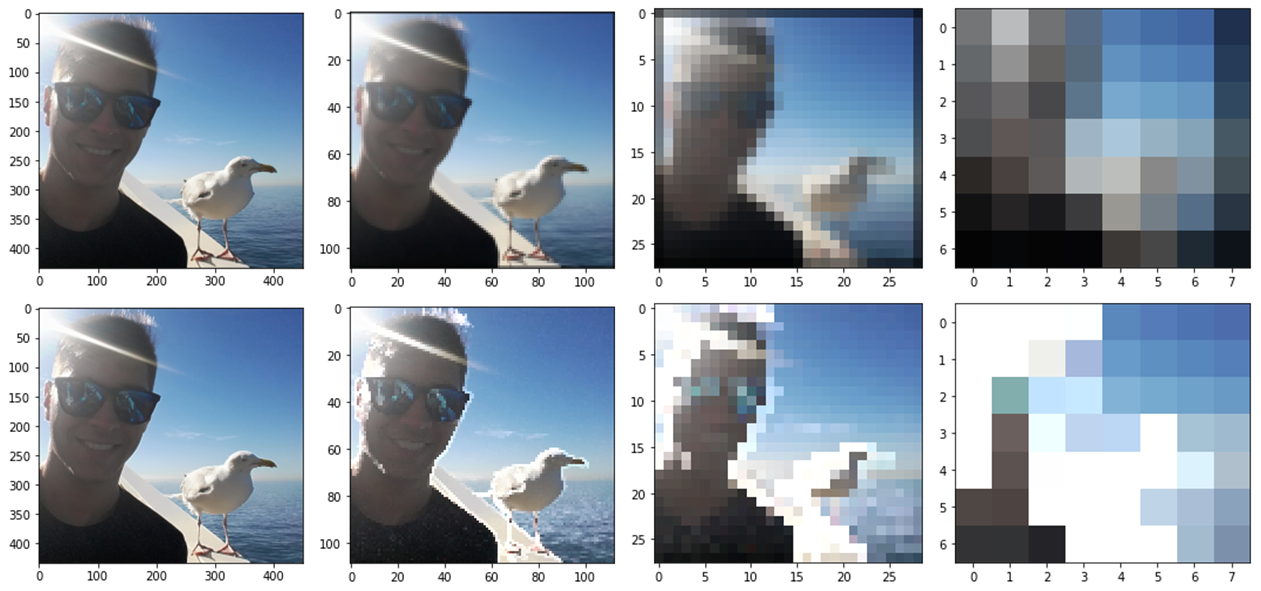
\includegraphics[width=1.0\columnwidth]{.//Figure/OCR/blur_vs_max_pool.png}}
 \caption{The effect of different pooling layers. The two variants were applied to the same $900\times865$ image eight times. The 2nd, 4th, 6th, and 8th downscaled images are shown. Blur-pooling was used with kernel size three and stride two (top) and max-pooling with stride two (bottom).}
 \label{fig:blur_vs_max_pool}
\end{figure}

\subsubsection{Predictor heads}

My implementation uses decoupled classifier- and localizer heads to produce the network output. I experimented with different input feature dimensions (coming from the FPN) and the number of layers.

I tried the predictor head input dimensions of \textit{256, 128}, and \textit{64}. The highest value matches the maximum dimensionality in the CNN backbone. Lower values can be interpreted as a feature downscaling in the FPN. Value 128 was the best choice because it could produce the best error rate in pair with dimension 256, leading to a significantly smaller network. Dimension 64 was too few for this problem. Table \ref{tab:predictor_head_dimension} summarizes the results.

\begin{table}[htb]
\caption{Comparison of predictor heads with different input dimensions.}
\label{tab:predictor_head_dimension}
\noindent
\centering
\begin{tabular*}
{\columnwidth}{@{\extracolsep{\stretch{1}}}*{3}{r}@{}}
    input dimension & epochs & loss\\ \hline
    64 & $22$ & $1.9347$ \\
    128 & $26$ & $\textbf{1.4033}$ \\
    256 & $28$ & $1.4052$ \\             
\end{tabular*}
\end{table}

RetinaNet uses two inner convolutional layers in the predictor heads before the last one reshaping the features to the output. I tried one, two, and three inner layers. A single layer was not enough. The loss was higher than with the other two approaches. The deepest predictor heads performed similar, but I chose the ones with two inner layers because of the similar performance but lower number of parameters. Results can be seen in Table \ref{tab:predictor_head_layers}.

\begin{table}[htb]
\caption{The effect of different number of inner predictor head layers on performance.}
\label{tab:predictor_head_layers}
\noindent
\centering
\begin{tabular*}
{\columnwidth}{@{\extracolsep{\stretch{1}}}*{3}{r}@{}}
    number of inner layers & epochs & loss\\ \hline
    1 & $20$ & $1.4456$ \\
    2 & $26$ & $1.4033$ \\
    3 & $22$ & $\textbf{1.3967}$ \\
\end{tabular*}
\end{table}

Sample inference results of the best model can be seen in Figure \ref{fig:inference_detector}. False positive predictions mainly cause the error. In the output processing, I used the Combined NMS algorithm with an IoU value of 0.5. To solve the false positive phenomenon, I could use the original NMS. Still, in that case, rotated images are likely to produce IoU values greater than the threshold among different objects, which carry the risk of dropping true positive objects close to each other. 

The TensorFlow Object Detection API model runs in 80 ms, while the proposed model's inference time is 317 ms. This phenomenon is caused by several things. The first is the number of anchor boxes. The API model uses around 12,000 anchor boxes, while the own implementation has four times more. This is because small anchor boxes are needed to detect small characters, drastically increasing the number of anchors. The other reason is that my implementation reuses the same predictor heads across different feature levels on the computational graph, leading to a smaller network size but longer inference time.

A development option could be to implement a YOLO-like detector, which uses objectness score to handle class imbalance, thus using a simpler, less parameter-sensitive loss function. Also, implementing an anchor-free version of the model could speed up inference time because the output tensor with roughly 50,000 items is a performance bottleneck. The model size can also be sacrificed using separate predictor heads for each feature level for better runtime.

\begin{figure}[htb]
 \centerline{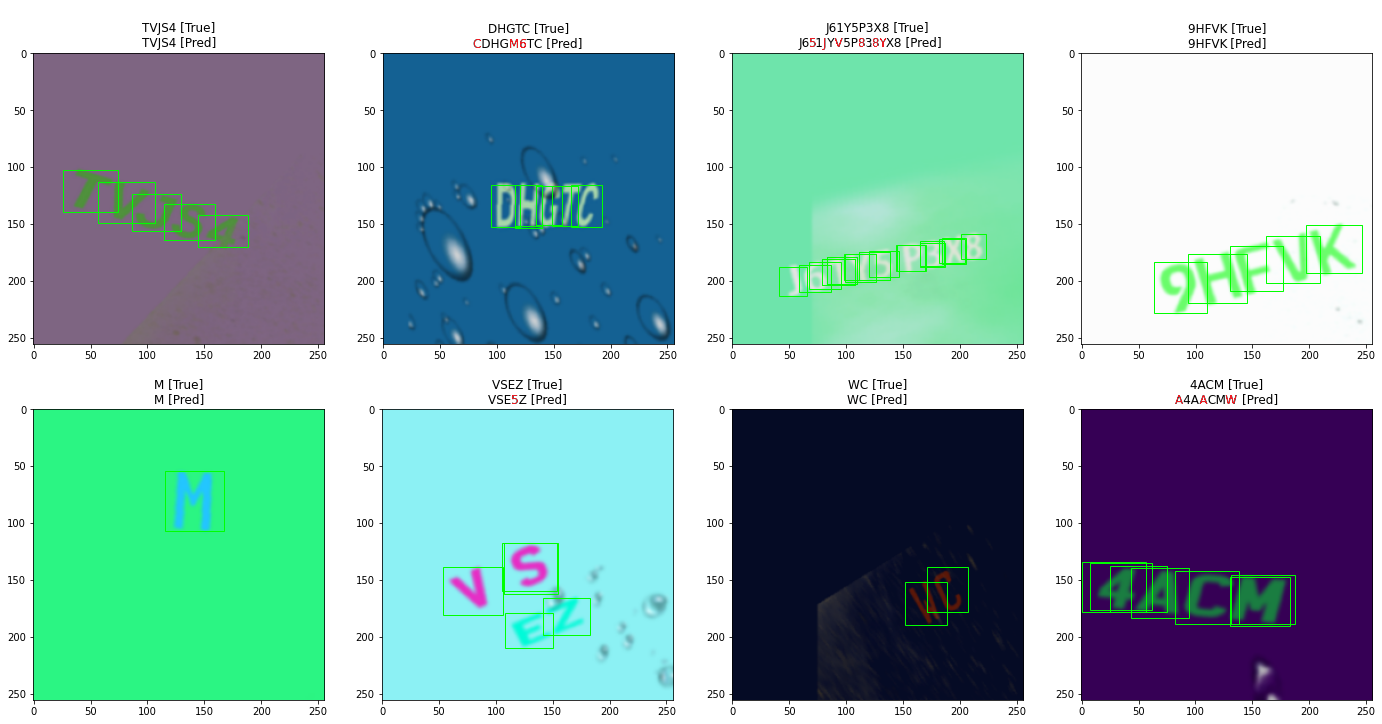
\includegraphics[width=1.0\columnwidth]{.//Figure/OCR/inference_detector.png}}
 \caption{Inference results of the best performing network. Incorrect detections are marked as red.}
 \label{fig:inference_detector}
\end{figure}

\section{Comparison}

This chapter provided a solution for the OCR task with both the sequential- and object detection approach. The sequential model is fast and simple but cannot process multiline texts efficiently. Object detection can handle them easily but requires roughly 2-3 times more parameters. However, its most significant problem is the inference time. With an anchor-free approach, the detector can be significantly faster, with which it can approach the runtime of the RCNNs. This is a future development opportunity. However, the present anchor-based detector is an order of magnitude slower than the sequential model, and more error prone due to the false positive predictions, so I chose the RCNN approach. The comparison of the two models can be seen in Table \ref{tab:sequential_detection_OCR_models}.

\begin{table}[htb]
\caption{Comparison of sequential and object detection OCR models.}
\label{tab:sequential_detection_OCR_models}
\noindent
\centering
\begin{tabular*}
{\columnwidth}{@{\extracolsep{\stretch{1}}}*{6}{r}@{}}
	model & host & input & parameters & size [KB] & inference [ms]\\ \hline
	sequential & CPU & 50x500x3 & $1,325,734$ & $639$ & $37$ \\
	object detection & CPU & 256x256x3 & $3,557,484$ & $4,541$ & $317$ \\
\end{tabular*}
\end{table}